\documentclass{standalone}
\usepackage{tikz}
\usetikzlibrary{arrows}
\begin{document}

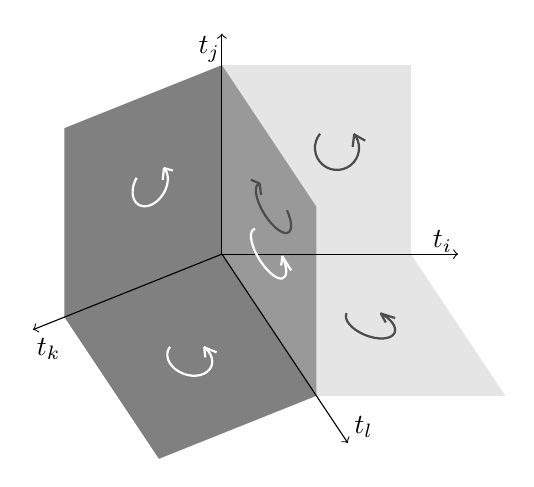
\begin{tikzpicture}[scale=(0.4),arrow/.style={->, >=angle 90,line width=.8pt}]
\fill[black!50!] (-5,-2) -- (-5,4) -- (0,6) -- (0,0) -- cycle;
\fill[black!10!] (0,6) -- (6,6) -- (6,0) -- (0,0) -- cycle;
\fill[black!50!] (-5,-2) -- (-2,-6.5) -- (3,-4.5) -- (0,0) -- cycle;
\fill[black!10!] (6,0) -- (9,-4.5) -- (3,-4.5) -- (0,0) -- cycle;

\fill[black!40!] (0,6) -- (0,0) -- (3,-4.5) -- (3,1.5) -- cycle;

\draw [->] (0,0) -- (7.5,0);
\draw [->] (0,0) -- (0,7);
\draw [->] (0,0) -- (-6,-2.4);
\draw [->] (0,0) -- (4,-6);

\def\warrow at (#1,#2) {
	\draw [line width=.8pt, white] (#1,#2) ++(140:5mm) arc (-220:40:7mm);
	\draw [line width=.8pt, white] (#1+.7,#2+.3) -- (#1+.65,#2-.1);
	\draw [line width=.8pt, white] (#1+.7,#2+.3) -- (#1+1.05,#2+.1);
}
\def\barrow at (#1,#2) {
	\draw [line width=.8pt, black!70!] (#1,#2) ++(140:5mm) arc (-220:40:7mm);
	\draw [line width=.8pt, black!70!] (#1+.7,#2+.3) -- (#1+.65,#2-.1);
	\draw [line width=.8pt, black!70!] (#1+.7,#2+.3) -- (#1+1.05,#2+.1);
}
%\warrow at (0,5)

	\barrow at (3.5,3.5)
\begin{scope}[cm={1,0,-.5,.7,(0,0)}]
	\barrow at (3,-3)
\end{scope}
\begin{scope}[cm={-.8,.8,0,.8,(0,0)}]
	\barrow at (-2.2,4)
\end{scope}
%\draw [arrow, black!70!] (5,-2) ++(140:5mm) arc (-220:40:7mm);

\begin{scope}[cm={.8,.3,0,.9,(0,0)}]
	\warrow at (-3,3.5)
\end{scope}
\begin{scope}[cm={1,0,-.2,.8,(0,0)}]
	\warrow at (-2,-4)
\end{scope}
\begin{scope}[cm={.8,-.8,0,.8,(0,0)}]
	\warrow at (1.7,2)
\end{scope}

\node at (7,.4) {$t_i$};
\node at (-.4,6.5) {$t_j$};
\node at (-5.5,-3) {$t_k$};
\node at (4.5,-5.5) {$t_l$};
\end{tikzpicture}
\end{document}